\section{Part IV - Kalman filter}
\begin{itemize}
    \item Introduce and motivate the task. You can include a brief summary of the different tasks in the lab-preparation assignment which was necessary to complete the lab. No extensive listing or derivation of equations are needed (you can mention, e.g., measurement noise, process noise, optimal estimator, etc.). 
    \item Include your hypothesis/test-plan and explain your thought process behind it.
    \item Include the results from the experiments that were done in the lab according to the test-plan, and any other tests you found interesting during your time in the lab (bonus tasks?). Include plots and discuss the result. This is the most important part of the report. How you structure this part of the report is up to you. 
    \item Conclusion. Include a short paragraph summarizing the results. 
\end{itemize}

The goal of this task is to implement and tune a Kalman filter, such that we get a stable system.
The matrices for the 6-state system looks like this:
\begin{equation}
    \begin{aligned}
        \mathbf{A}&=
        \begin{bmatrix}
            0 & 1 & 0 & 0 & 0 &0 \\
            0 & 0 & 0 & 0 & 0 & 0\\
            0 & 0 & 0 & 1 & 0 & 0\\
            0 & 0 & 0 & 0 & 0 & 0\\
            0 & 0 & 0 & 0 & 0 & 1\\
            K_3 & 0 & 0 & 0 & 0 & 0
        \end{bmatrix}\\
        \mathbf{B}&=
        \begin{bmatrix}
            0 & 0 \\
            0 & K_1 \\
            0 & 0 \\
            K_2 & 0 \\
            0 & 0 \\
            0 & 0
        \end{bmatrix}\\
        \mathbf{C}&=
        \begin{bmatrix}
            1 & 0 & 0 & 0 & 0 & 0 \\
            0 & 1 & 0 & 0 & 0 & 0\\
            0 & 0 & 1 & 0 & 0 & 0\\
            0 & 0 & 0 & 1 & 0 & 0\\
            0 & 0 & 0 & 0 & 0 & 1
        \end{bmatrix}\\
    \end{aligned}
\end{equation}

The discrete-time system is given with these matrices
\begin{equation}
    \mathbf{A_d}=\mathbf{A}\cdot t +\mathbf{I},\
    \mathbf{B_d}=\mathbf{B}\cdot t,\
    \mathbf{C_d}=\mathbf{C}
\end{equation}
\subsection{Hypothesis and test plan}
We will implement the kalmanfilter in simulink, and try out different values along the diagonal of $Q_d$. The test plan is shown in \autoref{tab:Kalmantestplan}. We will also apply external disturbances to test how the system handles that.

\begin{table}[htbp]
    \centering
    \caption{Test diagonal values in $Q_d$}
    \begin{tabular}{c|ccccc}
        \textbf{Test} & $Q_1$ & $Q_2$ & $Q_3$ & $Q_4$ & $Q_5$ \\
        \hline
        1 &0  & 0  & 0  & 0  & 0  \\
        2 &1000  & 1000  & 1000  & 1000  & 1000  \\
        3 &1  & 1  & 1  & 1  & 1  \\
    \end{tabular}
    \label{tab:Kalmantestplan}
\end{table}
Our hypothesis is that when all q values are 0, the filter will only follow the model. We also think that when all Q values are 1000, the filter will only follow the measurements. With all Q values set to 1, we believe we will obtain something in between, hopefully not too noisy.

\subsection{Results}
Our hypothesis was somewhat right. The edge cases of 0 and 1000 was right, but with Q values along 1, the estimated states were still wery noisy. Therefore we first tuned all diagonal values in Q toghether until we were somewhat satisfied with $\hat{x}$. This happend with $10^{-5}$. After that we tuned the different states seperately, and ended up with the $Q_d$ matrix shown in \autoref{eq:kalmanqmatrix}. Since we have no measurement of $\lambda$, we sat that value to 0.
\begin{equation}
    \begin{aligned}
        \mathbf{Q_d}&=
        \begin{bmatrix}
            10^{-6} & 0 & 0 & 0 & 0 & 0 \\
            0 & 10^{-5} & 0 & 0 & 0 & 0\\
            0 & 0 & 10^{-6} & 0 & 0 & 0\\
            0 & 0 & 0 & 10^{-5} & 0 & 0\\
            0 & 0 & 0 & 0 & 0 & 0\\
            0 & 0 & 0 & 0 & 0 & 10^{-4}
        \end{bmatrix}\\
    \end{aligned}
    \label{eq:kalmanqmatrix}
\end{equation}

In \autoref{fig:plotavkalman}, you can see the the different states in $\hat{x}$ compared to the IMU output while applying a lot of external disturbance. The kalman filter handles both IMU noise and external disturbances well.

\begin{figure}

    \centering
    \begin{subfigure}{0.40\textwidth}
      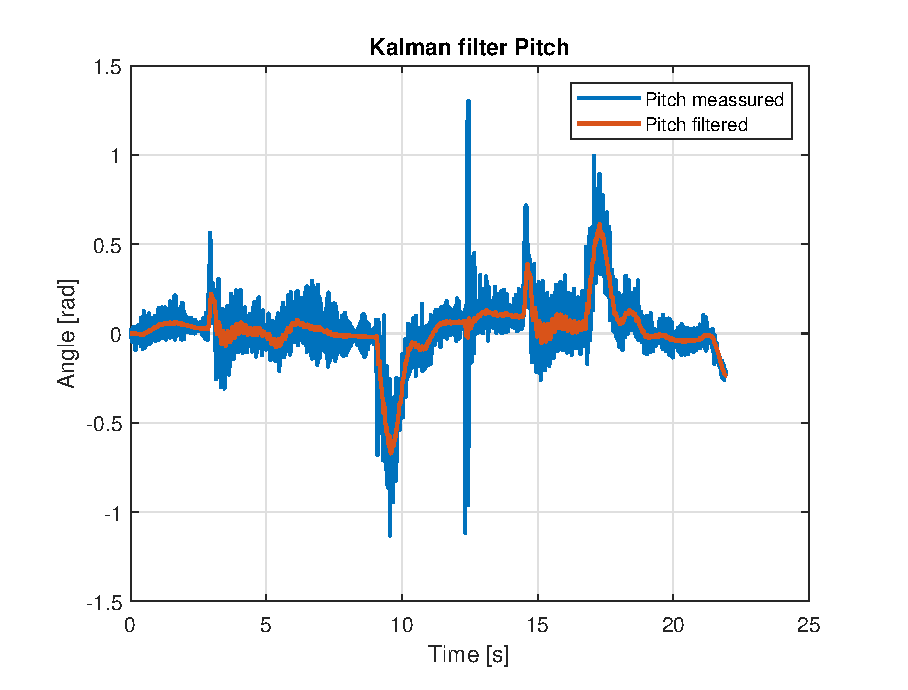
\includegraphics[width=\textwidth]{figures/labday4/p.eps}
      \caption{$p$}
    \end{subfigure}

    \begin{subfigure}{0.40\textwidth}
        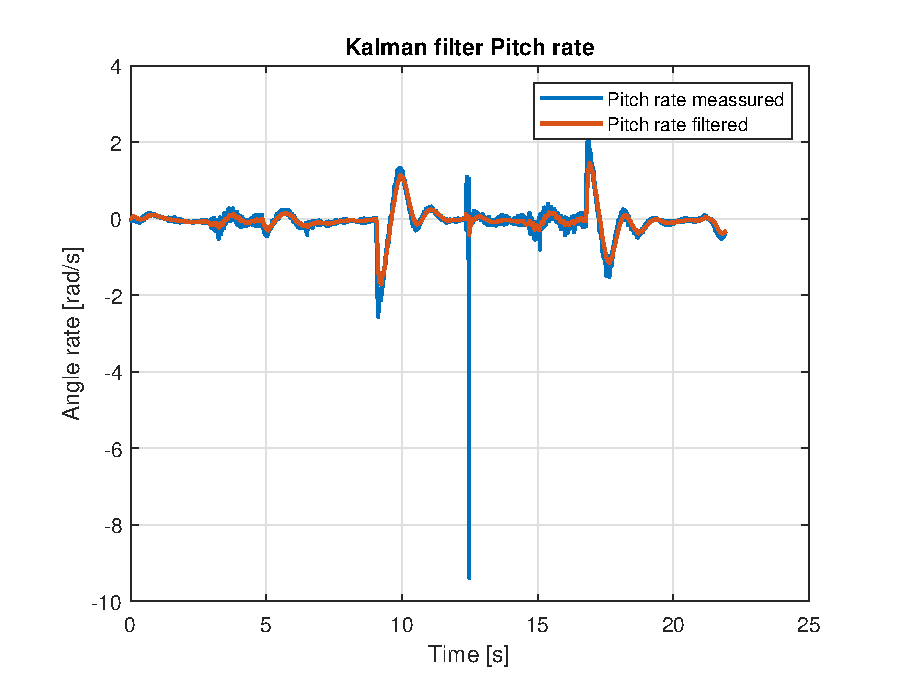
\includegraphics[width=\textwidth]{figures/labday4/p_dot.eps}
        \caption{$\dot{p}$}
    \end{subfigure}
    
    \begin{subfigure}{0.40\textwidth}
        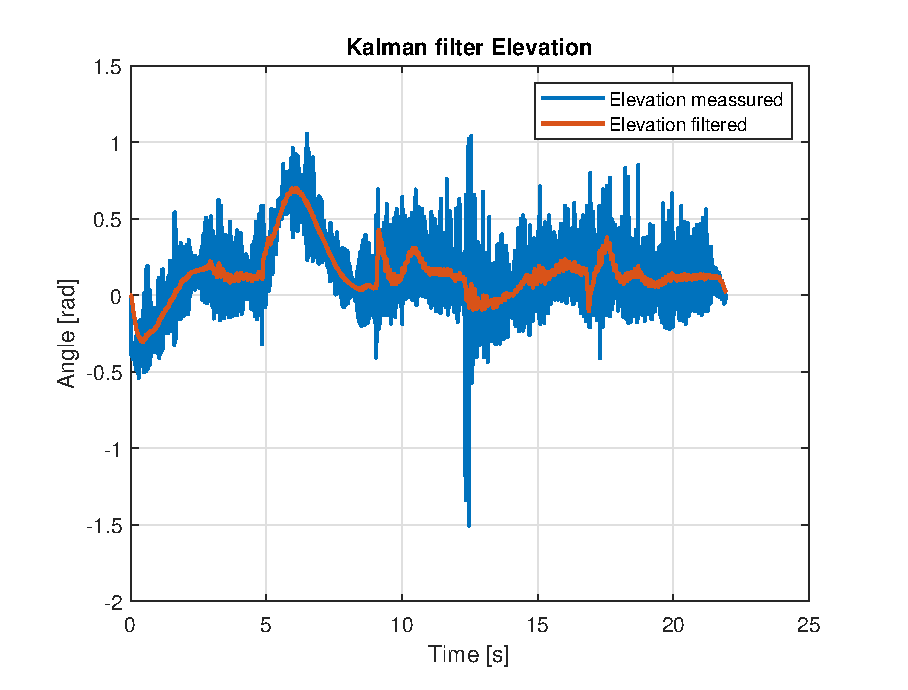
\includegraphics[width=\textwidth]{figures/labday4/e.eps}
        \caption{$e$}
    \end{subfigure}

    \begin{subfigure}{0.40\textwidth}
        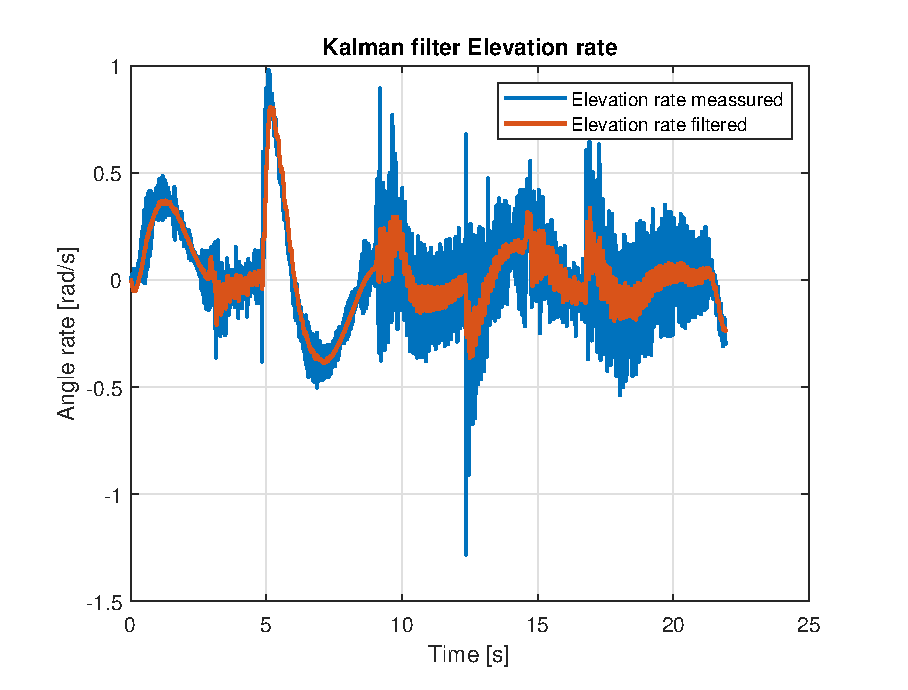
\includegraphics[width=\textwidth]{figures/labday4/e_dot.eps}
        \caption{$\dot{e}$}   
    \end{subfigure}
        
    \begin{subfigure}{0.40\textwidth}
        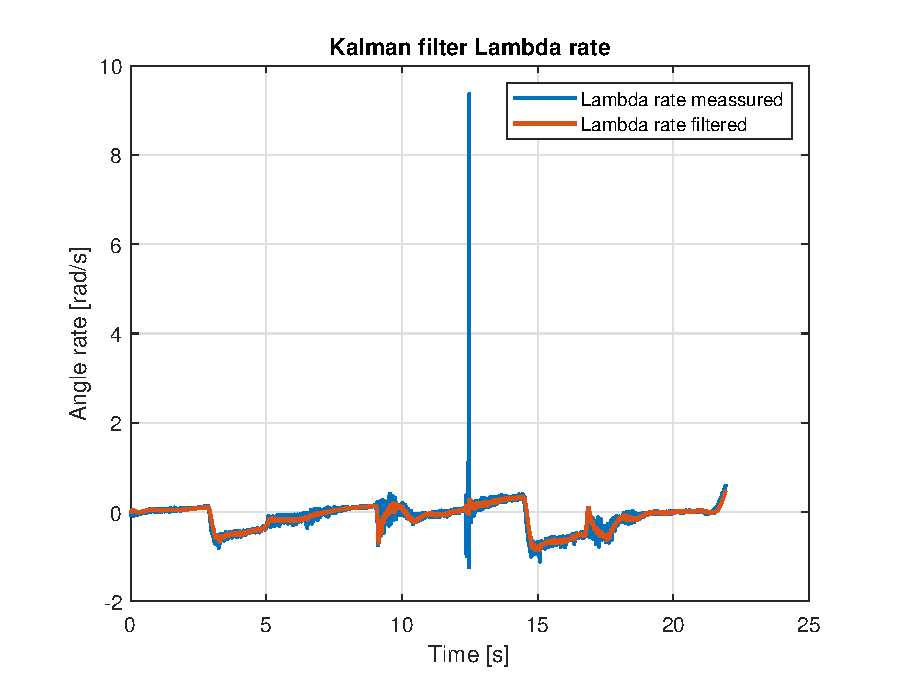
\includegraphics[width=\textwidth]{figures/labday4/lambda_dot.eps}
        \caption{$\dot{\lambda}$}
    \end{subfigure}
    
    \caption{Results for different poles}
    \label{fig:plotavkalman}
    
\end{figure}